% !Mode:: "TeX:UTF-8"
% 七年级上学期第一单元几何体的展开与折叠

\begin{defproblem}{7NJ-03-01}%
\begin{onlyproblem}%
(1) 研究几何体特征的思考顺序:

先研究\underline{\hspace*{2cm}},再研究\underline{\hspace*{2cm}}和\underline{\hspace*{2cm}}.

(2) 棱柱与棱锥的区别:

①底面不同:棱柱有\underline{\hspace*{2cm}}个底面,棱锥有\underline{\hspace*{2cm}}个底面;

②侧面不同:棱柱的侧面都是\underline{\hspace*{2cm}},棱锥的侧面都是\underline{\hspace*{2cm}}.

(3) 正方体的展开与折叠

①一个面与\underline{\hspace*{2cm}}个面相邻,与\underline{\hspace*{2cm}}个面相对;

②一条棱与\underline{\hspace*{2cm}}个面相连,一条棱被剪开成为\underline{\hspace*{2cm}}条边;

③一个顶点连着\underline{\hspace*{2cm}}条棱,一个点属于\underline{\hspace*{2cm}}个面.

(4) 利用三视图求几何体的表面积:

①\underline{\hspace*{2cm}};②\underline{\hspace*{2cm}}.
\end{onlyproblem}%
\begin{onlysolution}%
\begin{solution}%
(1) 面、棱和顶点.

(2) ①2,1;②长方形,三角形.

(3) ①4,1;②2,2;③3,3.

(4) ①作三视图;②注意凹陷部分.
\end{solution}%
\end{onlysolution}%
\end{defproblem}





\begin{defproblem}{7NJ-03-02}%
\begin{onlyproblem}%
如图所示的正方体的表面展开图可能是(    ) 
\begin{center}
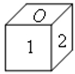
\includegraphics[width=1.5cm]{7NJ01-03-20190803-01.jpg}
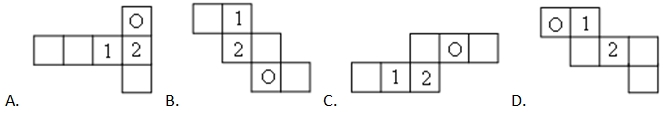
\includegraphics[width=9cm]{7NJ01-03-20190803-02.jpg}
\end{center}

\end{onlyproblem}%
\begin{onlysolution}%
\begin{solution}%%
A
\end{solution}%
\end{onlysolution}%
\end{defproblem}




\begin{defproblem}{7NJ-03-03}%
\begin{onlyproblem}%
如图是一个正方体的表面展开图,把它折起来,可以得到图中的(    ) 
\begin{center}
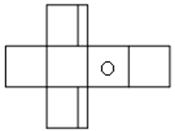
\includegraphics[width=2cm]{7NJ01-03-20190803-03.jpg}
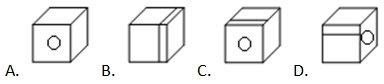
\includegraphics[width=7cm]{7NJ01-03-20190803-04.jpg}
\end{center}


\end{onlyproblem}%
\begin{onlysolution}%
\begin{solution}%%
C
\end{solution}%
\end{onlysolution}%
\end{defproblem}




\begin{defproblem}{7NJ-03-04}%
\begin{onlyproblem}%
将图1中的表面展开图还原为正方体,并按图2摆放,则图1中的线段MN在图2中的对应线段是(    ) 
\begin{center}
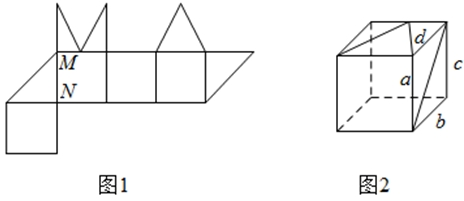
\includegraphics[width=7cm]{7NJ01-03-20190803-05.jpg}
\end{center}

\xx
{a}
{b}
{c}
{d}

\end{onlyproblem}%
\begin{onlysolution}%
\begin{solution}%%
C.
如图,   分析可得图1中的棱ME与图2中棱AD重合,因此面MNEF与面ABCD重合,所以图1中的线段MN是图2中面ABCD上的一条棱,只有c符合题意,故选C. 
\begin{center}
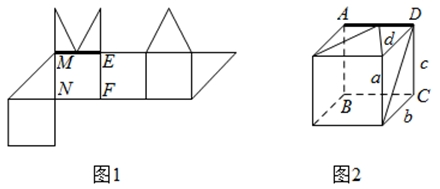
\includegraphics[width=7cm]{7NJ01-01-20190804-32}
\end{center}
\end{solution}%
\end{onlysolution}%
\end{defproblem}









